\documentclass[border=4pt]{standalone}
\usepackage{tikz}
\usetikzlibrary{calc,shapes.geometric}

\begin{document}
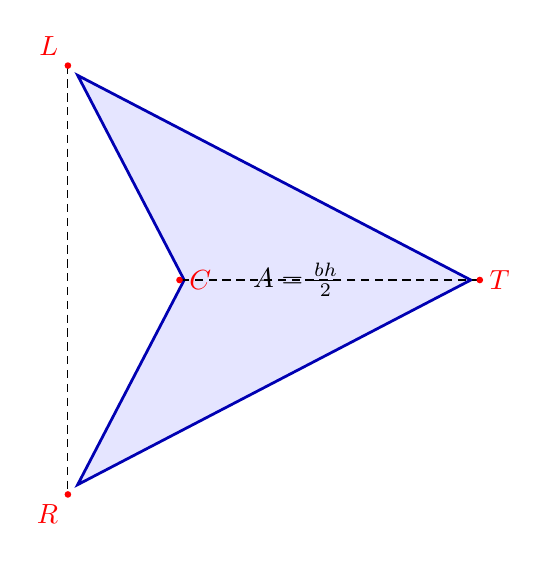
\begin{tikzpicture}
  \node[dart,dart tip angle=55,dart tail angle=125,
    minimum width=34mm,minimum height=50mm,draw=blue!70!black,
    fill=blue!10,line width=1pt,outer sep=1.5pt] (D) at (0,0) {};
  \draw[densely dashed] (D.tip) -- (D.tail center);
  \draw[densely dashed] (D.left tail) -- (D.right tail);
  \fill[red] (D.tip) circle (1.2pt) node[right] {$T$};
  \fill[red] (D.left tail) circle (1.2pt) node[above left] {$L$};
  \fill[red] (D.tail center) circle (1.2pt) node[right] {$C$};
  \fill[red] (D.right tail) circle (1.2pt) node[below left] {$R$};
  \node at ($(D.center)+(5mm,0)$) {$A=\frac{bh}{2}$};
\end{tikzpicture}
\end{document}
